\documentclass[a4paper,11pt]{article}

\input ../include/preamble.tex

\usepackage{tikz}
\usetikzlibrary{automata,arrows,topaths,calc,positioning}


\begin{document}


\title{
    \textbf{Monte Carlo and $\Pi$}\\
    \large{Programming II}
}
\author{Johan Montelius}
\date{Spring Term 2023}
\maketitle
\defaultpagestyle


\section*{Introduction}

You all know that $\pi$ is sort of $3.141592...$ but how do you
calculate a better approximation? Archimedes knew that $\pi$ was
slightly smaller than $22/7$ but was not sure about the third
decimal. Zu Chongzhi could narrow it down to $355/113$ wich is correct
to the sixth decimal. Your task is to compute a better approximation
using something called Monte Carlo method.

\section*{What do we know}


The Monty Carlo method is surprisingly simple and builds on that we
can generate a sequence of random numbers and that we know the
Pythagorean theorem.

Take a look at Fig.\ref{fig:pyth}, we have an arch with radious $5$
and a dot at $(2,3)$. If I ask you if the dot is inside our outside
the area limited by the arch you would of course say that it is
inside, but how do you prove this without looking at the picture?

One way is to use the Pythagorean theorem and show that the distance
from origo to the dot is $\sqrt{2^2 + 3^2} = 3.6..$ which is less than
$5$. This is trivial but how would it help us finding a good aproximation of $\pi$? 


\begin{figure}[h]
\center
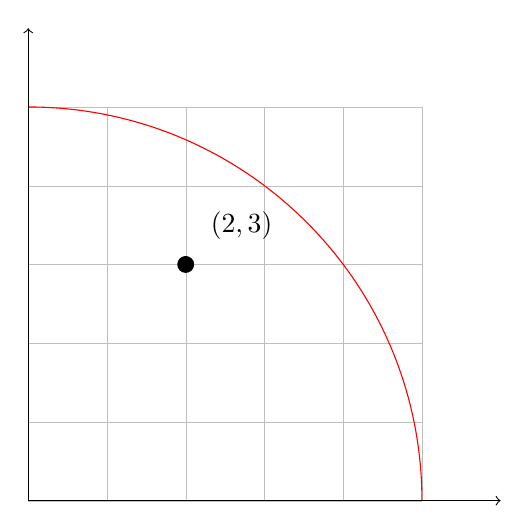
\begin{tikzpicture}
  \draw[lightgray,ultra thin] (0,0) grid (5,5);
  \draw[red] (5,0) arc (0:90:5);
  \draw[->] (0,0) -- (0,6);
  \draw[->] (0,0) -- (6,0);
  \node[] (dot) at (2,3){};
  \draw[fill=black] (dot) circle (1mm);
  \node[anchor = south west, above right = 0.1cm of dot] {$(2,3)$};
\end{tikzpicture}
\caption{Does (3,4) fall inside the circle?}
\label{fig:pyth}
\end{figure}


The trick is to look at the size of the area "inside" the arch
(i.e. the sector limited by the x and y axis and the arch) and compare this to
the area of the square limited by origo and the upper right corner at
$(5,5)$.

The square of course has an area of $5^2$ and the sector an area of
$(\pi/4) * 5^2$ and this is where $\pi$ comes into the picture.

\section*{A random dart}

If you throw a thound random darts at the square, how many would you
estimate hit the arch sector? The ratio would of course be proability
that a dart hits inside the arch is $\pi/4$ or aproximate $785$
darts. We know this since we know a good aproximation of $\pi$ but if
we didn't we could .... throw a thousand darts and count how many hit
inside the arch (and you know how to determine this).

If we throw a thousand darts and $782$ land inside the arch you would
estimate $pi$ to be $4*785/1000 = 3.140$ which of course is quite
close. You could of course and up with $782$ darts inside the arch and
estimate $\pi$ to be $3.128$. You would not know which one was closes
to the truth but if you throw ten thousand darts you woudl probably be
able to estimate $\pi$ with a better value.

This is how the Monte Carlo method or simulation works; do a serie of
experiments (on a computer) and try to aproximate what would be very
difficult to calculate. 

\section*{The challenge}


In order to find a good estimate of $\pi$ you need to set up a program
that throws more and more darts at a square and continiusly estimates
a value for $\pi$. As more darts are thrown you will see this estimate
fluctuate less and less and slowly converge. The challenge is to beat
the estimtes found by Archimedes, two decimals, and Zu Chongzhi, six
decimals.

You need a function can throw a random dart and tell you wether it hit
inside the arch or not. To your help you have a function {\tt
  Enum.random/1} that will give you a random number in a given
range. For example {\tt Enum.random(0..10)} will give you a number
between $0$ and $10$).  The function {\tt dart/1)} should take a
number, the radious $r$, and return true or false a randomly thrown
dart.

Now when we check if we are inside the arch we could of course
calculate $\sqrt{x^2 + y^2}$ and compare it to $r$ but we might as
well compare $x^2 + y^2$ to $r^2$. It's the same you say but there is
a difference. We avoid doing an expensive root calculation and we
avoid any problems with how floating point numbers are represneted
(whoch would not be a problem in this exercise). Use the function {\tt
  :math.pow/2} to caculate the square.

\begin{minted}{elixir}
  def dart(r) do
    x = Enum.ranomd(0..r)
    y = Enum.ranomd(0..r)
    ...  >  ... + ... 
  end
\end{minted}

Once we can throw one dart we throw a hundred or a thousand but since
we want to know how our estimate comes closer and closer to the true
value we trow a number of darts, called a round, and accumulate how
many that land inside the acrch. Define a function {\tt round/3} that
throws a number of darts, $k$, on a target with radious $r$ and add
the hits to the accumulated value $a$.

\begin{minted}{elixir}
  def round(0, _, a) do ... end
  def round(k, r, a) do
    if ... do
      round(..., ..., ...)
    else
      round(..., ..., ...)	
    end
  end
\end{minted}

Now you're fit to set up a test where you run a number of rounds and
display the estimated value for $\pi$ after each round. You can
compare the estimate to {\tt :math.pi()} to see how far off your are.


\begin{minted}{elixir}
  def rounds(k, j, r)  do
    rounds(k, j, 0, r, 0)
  end
  
  def rounds(0, _, t, _, a) do ...  end
  def rounds(k, j, t, r, a) do
    a = round(j, r, a)
    t = t + j
    pi = ...
    :io.format(" ... ", [pi, (pi - :math.pi()])
    rounds(k-1, j, t, r, a)
  end
\end{minted}

Do some experiments and try to beat Archimedes. How many darts do you
need before your can for sure state that you have better value; how
would you know if you did not have {\tt :math.pi()}?

Try to beat Zu Chongzhi; note that you now have to produce a value
that is accurate to the sixth decimal. It means that you will have to
throw many millions of darts. If you only throw a hundredthousand
darts you will, if you're lucky, find $78.540$ dars inside the arch
and guess that $\pi = 3.14159$ but you will not get closer than this.

It also means that your discrete radious, $r$, needs to be suffienctly
large to captue the difference in the sixth decimal. If you only have
a radius of $1 000$ and thus have $1 000 000$ points to examine, you
will not get closer than $3.14159$ even if you throw all darts.

Since you will need to throw a slot of darts you  might
want to modify the definition of {\tt rounds/5} so that it doubles the
number of dart throwns i each round.

How close do you come, what is you best estimate of $\pi$?

\section*{Summary}

All though a fun exercise, the Monte Carlo method is not used to
estimate the value of $\pi$. As you probably learned it takes for ever
to find an aproxiamtion with more than five accurate decimals. There
are more efficiet ways to calculate $\pi$, for example summing up the
Leibniz formula:

$$\pi/4 = 1 - 1/3 + 1/5 - 1/7 + 1/9 - ... $$

Try:

\begin{minted}{elixir}
  4 * Enum.reduce(0..1000, 0, fn(k,a) -> a + 1/(4*k + 1) - 1/(4*k + 3) end)
\end{minted}

The idea with Monte Carlo is to get a rough estimate of somthing that
i to complicated to calculate. As you saw you could get a an
aproximation of $3.1$ or $3.2$ in only a few darts and it might be
sufficent to have an idé of a value with a error margin of a couple of
percent if the alternative is to know nothing at all.


  

\end{document}
